\documentclass[12pt,a4paper]{article}
\usepackage[utf8]{inputenc}
\usepackage[spanish]{babel} % Para modificar labels por defecto
\usepackage[bottom]{footmisc} % Para las notas al pie de la página
\usepackage[T1]{fontenc}
\usepackage{siunitx}
\usepackage{tocbibind} % Bibliografía en el indice
\usepackage{titlesec} % Posibilidad de editar los formatos de chapter
\usepackage{amsmath,amssymb,mathrsfs} % Matemáticas varias
\usepackage{tabularx} % Para las tablas
\usepackage{fancyhdr}
\renewcommand{\baselinestretch}{1} % Interlineado. 1 es estandar
% --- Arreglos varios para la inclusion de imagenes
\usepackage{float}
\usepackage[pdftex]{graphicx}
\graphicspath{{T:/Tom/Facultad/Materias/arqui/Practico/tp3/informe/imgs/} {T:/Tom/Facultad/Logos/}}
\usepackage{subfigure}
\usepackage[usenames,dvipsnames]{color}
\DeclareGraphicsExtensions{.png,.jpg,.pdf,.mps,.gif,.bmp}
% --- Para las dimensiones de los márgenes etc
\frenchspacing \addtolength{\hoffset}{-1.5cm}
\addtolength{\textwidth}{3cm} \addtolength{\voffset}{-2.5cm}
\addtolength{\textheight}{4cm}
% --- Para el encabezado
\setlength{\headheight}{33pt}

\fancyhead[R]{\includegraphics[height=1cm]{logo_fcefyn_nuevo.jpg}}
\fancyhead[L]{\includegraphics[height=1cm]{unc1_a.jpg}}
\fancyhead[C]{}
\fancyfoot[C]{Página \thepage} \renewcommand{\footrulewidth}{0.4pt}
\pagestyle{fancy}

% --- Para las tablas
\usepackage{multirow} % Juntar filas
\newcolumntype{L}[1]{>{\raggedright\arraybackslash}p{#1}} % Justificar Izq
\newcolumntype{C}[1]{>{\centering\arraybackslash}p{#1}} % Justificar Centrar
\newcolumntype{R}[1]{>{\raggedleft\arraybackslash}p{#1}} % Justificar Der
\usepackage[numbered]{bookmark} % Para que figure las secciones en el PDF
\usepackage{listings} % Para poner código
\usepackage{enumitem} % Para editar las propiedades de los items
\lstset{frame=single} % Código en un cuadro

% --- Quita los cuadrados de colores en los hipervínculos
\hypersetup{
	colorlinks  = true,
	linkcolor   = black,
	urlcolor    = black,
  	citecolor   = black,
  	filecolor   = black,
  	anchorcolor = black}

% --- Para cambios de nombres
\addto\captionsspanish{%
  \renewcommand\tablename{Tabla}
}

% -------------------------------------------------------- %
% Definicion de colores para el codigo

\lstset{
    literate={á}{{\'a}}1
        {ã}{{\~a}}1
        {é}{{\'e}}1
        {ó}{{\'o}}1
        {í}{{\'i}}1
        {ñ}{{\~n}}1
        {¡}{{!`}}1
        {¿}{{?`}}1
        {ú}{{\'u}}1
        {Í}{{\'I}}1
        {Ó}{{\'O}}1
}

\lstdefinelanguage{ve}{
  backgroundcolor=\color{white},		%color de fondo
  commentstyle=\color{CadetBlue},		%color de los comentarios
  keywordstyle=\color{Plum},			%color de las palabras reservadas
  numberstyle=\tiny\color{ForestGreen},	%numero de línea con tamaño y color
  numbers=left,                    	%posicion de los numeros
  numbersep=5pt,   					%espaciado entre los numeros
  stringstyle=\color{OliveGreen},		%color de las strings
  basicstyle=\ttfamily\footnotesize,	%estilo de fuente
  breakatwhitespace=false,         	%romper estacios en blanco
  breaklines=true,                 	%romper lineas
  frame=single,						%para encuadrar el codigo
  rulecolor=\color{black},			%color del cuadro
  showspaces=false,
  showstringspaces=false,
  showtabs=false,
  tabsize=2,
  language=Verilog
}

\renewcommand{\lstlistingname}{Código}

% -------------------------------------------------------- %
%Para subsubsubsection

\usepackage{titlesec}
\titleformat{\paragraph}
{\normalfont\normalsize\bfseries}{\theparagraph}{1em}{}
\titlespacing*{\paragraph}
{0pt}{3.25ex plus 1ex minus .2ex}{1.5ex plus .2ex}

% -------------------------------------------------------- %
\begin{document}

\begin{titlepage}
    \begin{center}
      \vspace*{1cm}

      \vspace{2cm}
      \includegraphics[width=0.4\textwidth]{unc1_a.jpg}
      \includegraphics[width=0.4\textwidth]{logo_fcefyn_nuevo.jpg}

      \Huge
      \textbf{Cátedra de Arquitectura de Computadoras}

      \vspace{3.5cm}

      \textbf{Trabajo Práctico N\si{\degree} III}\\
      \textbf{BIP I}

      \vfill

      \vspace{0.8cm}



      \Large
      Carrizo, Aixa Mariel\\
      Piñero, Tomás Santiago\\      
      10 de Diciembre de 2020
    \end{center}
\end{titlepage}
% -------------------------------------------------------- %
% --- Tabla de contenidos

\setcounter{secnumdepth}{4}
\setcounter{tocdepth}{5}
\tableofcontents

% -------------------------------------------------------- %

\newpage
\renewcommand{\baselinestretch}{1}
\setlength{\parskip}{0.5em}


\newpage
\section{Enunciado}
\label{sec:enun}

El objetivo de este trabajo es implementar en FPGA, programando en Verilog, un procesador monociclo sin saltos. Este procesador se encuentra explicado detalladamente en \cite{bip} como ``BIP I''. 
Los requerimientos del trabajo son los siguientes:

\begin{itemize}[leftmargin=1.5cm, itemsep=1pt]
\item Se debe ejecutar una instrucción por ciclo de reloj;
\item Se deben implementar las instrucciones de la Tabla \textbf{\ref{tab:bipi}}.
\item Al ejecutar una instrucción \verb|HLT|, se debe transmitir el valor del
acumulador;
\item Validar el desarrollo por medio de \emph{Test Bench}.	
\end{itemize}

\subsection{Arquitectura del procesador}
\label{subs:arqui}

El BIP soporta direccionamientos directo e indirecto, con un bus de 16 bits tanto para datos (números enteros) como para instrucción.

Las instrucciones están conformadas por dos campos:

\begin{enumerate}
\item \textbf{Código de operación}: Los 5 bits más significativos. Indica qué instrucción se va a ejecutar;
\item \textbf{Operando}: Los 11 bits menos significativos. Indica el operando para la instrucción, que puede ser un dato inmediato (un número constante) o una dirección del dato en la memoria (una variable).
\end{enumerate}

En la siguiente Tabla se muestran las instrucciones junto con su código, mnemónico y la actualización de la memoria de datos (DM) y el acumulador (ACC). 
El contador de programa se aumenta en 1 en cada ejecución de instrucción, con excepción de \emph{`Halt'}.

\begin{table}[H]
\centering
\begin{tabular}{||l|c|c|l||}
\hline
\multicolumn{1}{||c|}{\textbf{Instrucción}} & \textbf{Codigo} & \textbf{Mnemonico} & \multicolumn{1}{c||}{\textbf{Actualización de ACC y DM}} \\ \hline
Halt                                       & 00000           & HLT                & \multicolumn{1}{c||}{-}                                       \\ \hline
Store Variable                             & 00001           & STO                & DM{[}operando{]} $\leftarrow$ ACC                            \\ \hline
Load Variable                              & 00010           & LD                 & ACC $\leftarrow$ DM{[}operando{]}                            \\ \hline
Load Immediate                             & 00011           & LDI                & ACC $\leftarrow$ operando                                    \\ \hline
Add Variable                               & 00100           & ADD                & ACC $\leftarrow$ ACC + DM{[}operando{]}                      \\ \hline
Add Immediate                              & 00101           & ADDI               & ACC $\leftarrow$ ACC + operando                              \\ \hline
Subtract Variable                          & 00110           & SUB                & ACC $\leftarrow$ ACC - DM{[}operando{]}                      \\ \hline
Subtract Immediate                         & 00111           & SUBI               & ACC $\leftarrow$ ACC - operando                              \\ \hline
\end{tabular}
\caption{Instrucciones del BIP I.}
\label{tab:bipi}
\end{table}

\begin{figure}[H]
\centering
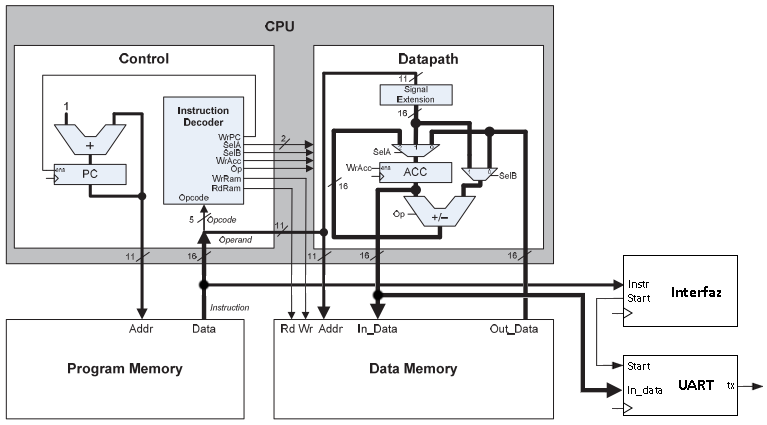
\includegraphics[scale=0.8]{tp3-bip.png}
\caption{Esquema del proyecto.}
\label{fig:esq}
\end{figure}

\section{Desarrollo}
\label{sec:des}

\subsection{Diseño}
\label{subs:diseño}

Se siguió el diseño propuesto en la Figura \textbf{\ref{fig:esq}}. La CPU está conformado por dos módulos:

\begin{itemize}
\item \textbf{Control}: toma las instrucciones de la memoria de programa, las decodifica y manda las operaciones al bloque \emph{datapath}. Está compuesto por:

	\begin{itemize}
	\item registro de contador de programa (PC);
	\item sumador de 11 bits;
	\item decodificador combinacional.
	\end{itemize}

\item \textbf{\emph{Datapath}}: procesa los datos bajo el comando del bloque de control. Tiene:

	\begin{itemize}
	\item registro de ACC;
 	\item suma y resta de 16 bits;
 	\item extensor de bits;
 	\item dos multiplexores.
	\end{itemize}
\end{itemize}

Este módulo interactúa con los módulos de memoria, uno para el programa y otro para los datos.

Para comunicar la CPU con el UART, se diseñó una interfaz que controla el contador de programa para indicar el envío del acumulador.

\subsubsection{Bloque de control}
\label{subss:control}

El bloque de control trabaja en los flancos positivos del \emph{clock}, instancia el módulo \emph{`op\_decoder'} y modifica el contador de programa de acuerdo a la salida \verb|o_write_pc| del mismo.
Consta de una entrada (\verb|i_instruction|) y 8 salidas:

\begin{enumerate}
\item \verb|o_operand|: operando de la instrucción.
\item \verb|o_sel_a|: selección del multiplexor A (memoria, operador o resultado de la alu)
\item \verb|o_sel_b|: selección del multiplexor B (memoria u operador).
\item \verb|o_write_acc|: escribir el acumulador.
\item \verb|o_operacion|: operación a realizar (suma o resta).
\item \verb|o_write_ram|: escribir la memoria de datos.
\item \verb|o_read_ram|: leer la memoria de datos.
\item \verb|o_addr|: leer la siguiente instrucción.
\end{enumerate}

\textbf{Decodificador de operación}

Este módulo se encarga de tomar los 5 bits más significativos de la instrucción de entrada (\verb|i_instruction|) y decodifica la operación a realizar junto con los datos a utilizar. 

Los códigos de las operaciones son los que se muestran en la Tabla \textbf{\ref{tab:bipi}}.

\subsubsection{\emph{Datapath}}
\label{subss:datapath}
Este módulo lee/escribe la memoria de datos y realiza las operaciones según las instrucciones que recibe del bloque de control durante los flancos negativos del \emph{clock}.

Como recibe un operando de 11 bits (\verb|i_operando|) y el procesador trabaja con 16, lo primero que se realiza es una extensión del signo del operando ingresado.

Para facilitar el entendimiento de código se usaron parámetros locales que indican los valores que deben seleccionar los multiplexores:

\begin{itemize}
\item \verb|MEMORIA|: se debe utilizar el valor desde la memoria de datos;
\item \verb|OPERANDO|:  se debe utilizar el operando de la instrucción;
\item \verb|RESULTADO|: se debe utilizar el resultado de la operación realizada.
\end{itemize}

\subsubsection{\emph{bip\_i}}
\label{subss:bipi}
Instancia los dos módulos explicados anteriormente. Su objetivo es verificar el correcto funcionamiento del procesador (ver Sección \textbf{\ref{subs:tb}}).

\newpage
\subsubsection{Memorias}
\label{subss:memo}
Para los módulos de memoria se utilizó la plantilla provista por Vivado. Se trata de un bloque de memoria RAM \emph{`No change mode'}, que es el recomendado para consumir poca potencia.

La plantilla se encuentra en:

\begin{center}

\footnotesize
\texttt{Templates $\rightarrow$ Synthesis Constructs $\rightarrow$  Example Modules $\rightarrow$  RAM $\rightarrow$ BlockRAM $\rightarrow$ Single Port}

\end{center}

La memoria de datos trabaja en el flanco positivo del \emph{clock}, mientras que la de programa trabaja en el flaco negativo.

\subsubsection{Interfaz}
\label{subss:iface}
Este módulo se encarga de monitorear la instrucción leída por el procesador cada vez que se detecta un cambio en el \emph{wire}. En caso de ser una instrucción \verb|HLT|, le indica al transmisor UART que envíe el valor que se encuentra actualmente en el acumulador. Su código es el siguiente:

\begin{lstlisting}[caption={Código fuente de ``interfaz\_uart''.}, label={cod:int-src}, language=ve]
`timescale 1ns / 1ps

module interfaz_uart
(
    input  wire [15:0] i_instruccion,
    input  wire        i_valid,
    output wire        o_tx_start
);

    localparam [15:0] HLT = 16'b0;

    reg tx_start;
    
    assign o_tx_start = tx_start;
    
    always@(*)begin:check
        tx_start = 1'b0; 
        
        if(i_valid)
        begin
            if(i_instruccion == HLT)
                tx_start = 1'b1;
            else
            	tx_start = 1'b0;
        end        
    end
endmodule
\end{lstlisting}

\newpage
\subsubsection{UART}
\label{subss:uart}
Se utilizaron los módulos \verb|tx_uart| y \verb|baudrate_generator| del trabajo práctico anterior.

La única diferencia con el anterior es que esta vez el parámetro \verb|DATA_BITS| vale 16 en vez de 8.


\subsubsection{\emph{top}}
\label{subss:top}
Es el módulo que instancia todos los módulos anteriores. El resultado de los \emph{testbenches} realizados se muestran a continuación.

\subsection{\emph{Testbench}}
\label{subs:tb}

\begin{figure}[H]
	\centering
	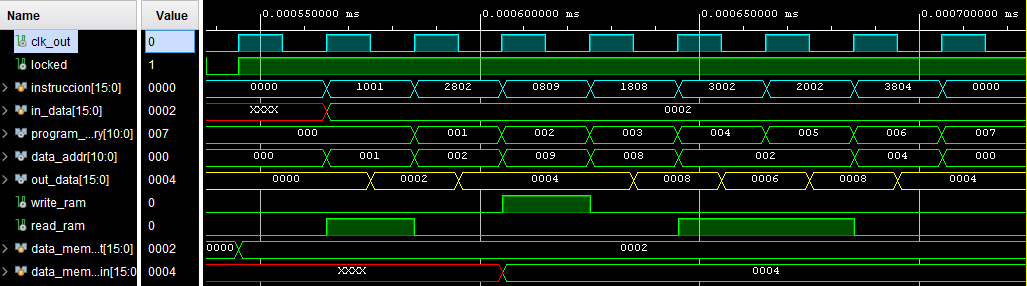
\includegraphics[width=16cm]{bip_sim.png}
	\caption{Resultado de \emph{`tb\_bip'}.}
	\label{fig:bip}
\end{figure}

En la Figura \textbf{\ref{fig:bip}} se muestra la ejecución del \emph{testbench} procesador (bip\_i) con estas instrucciones:

\begin{lstlisting}[language=ve]
  16'b00010_000_0000_0001; // Load variable 0x01 => ACC=DRAM[0x01]
  16'b00101_000_0000_0010; // Add immediate +0x2 => ACC=DRAM[0x01]+0x02
  16'b00001_000_0000_1001; // Store in 0x9 =>DRAM[0x09]=ACC
  16'b00011_000_0000_1000; // Load immediate 0x08 => ACC=0x08
  16'b00110_000_0000_0010; // Substract variable in 0x02 => ACC=0x08-DRAM[0x02]
  16'b00100_000_0000_0010; // Add variable in 0x02 => ACC=0x08
  16'b00111_000_0000_0100; // Substract immediate 0x04 => ACC = 0x04
  16'b00000_000_0000_0000; // Halt
  16'b00010_000_0000_0001; // Load variable 0x01 => ACC=DRAM[0x01]
\end{lstlisting}

Luego, la simulación con tiempo del módulo \emph{top} dio el siguiente resultado:

\begin{figure}[H]
	\centering
	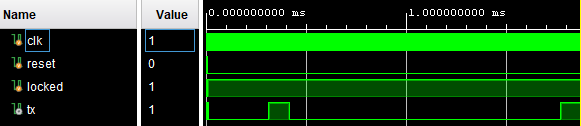
\includegraphics{top_sim.png}
	\caption{Resultado de \emph{`tb\_top'}.}
	\label{fig:top}
\end{figure}


\section{Cálculo de frecuencia máxima}
\label{sec:freq}

Para obtener el valor de la máxima frecuencia a la que puede trabajar el
circuito se utilizó el reporte de tiempo que provee Vivado. Para obtener este reporte se deben hacer los siguientes pasos:

\begin{enumerate}
\item Dirigirse a la opción `\emph{Edit timing constraints}';
\item Seleccionar `\emph{Create clock}' y crear uno nuevo;
\item Agregar como `\emph{source object}' la entrada del \emph{clock} del diseño realizado;
\item Definir la frecuencia del \emph{clock}.
\end{enumerate}

Una vez hecho esto, el reporte de tiempo realizado por Vivado muestra 
que el tiempo de \emph{setup} es de \verb|1.327 [ns]| y el tiempo de \emph{hold} es de \verb|0.232 [ns]|.

Sumando estos tiempos, se obtiene el tiempo del \emph{clock}:
\begin{align*}
	t_{clock} &= t_{setup} + t_{hold} \\
	t_{clock} &= 1.327 + 0.232 \\
	t_{clock} &= 1.559\,[ns]
\end{align*}

Finalmente, el periodo del \emph{clock} es:

\begin{equation}
f_{clock} = 641\,[MHz]
\end{equation}

\section{Conclusiones}
\label{concu}

Se logró implementar un diseño modularizado del modelo propuesto, que permitió encontrar los errores con más facilidad cuando las simulaciones no mostraban los resultados esperados.

Se incorporó la utilización de herramientas de análisis de tiempo provistas por Vivado, lo que facilitó el cálculo de la frecuencia máxima de operación del circuito.

\begin{thebibliography}{9}

\bibitem{bip}
Maicon Carlos Pereira, Paulo Viniccius Viera, André Luis Alice Raabe and Cesar Albenes Zeferino. \emph{A Basic Processor for Teaching
Digital Circuits and Systems Design with FPGA}. University of Vale do Itajai, 2012 \\

\end{thebibliography}
\end{document}